\chapter{Game Design Document}
\label{chap:gdd}

Como se explicaba en el \autoref{chap:stateofart}, el \textit{Game Design Document} (GDD) es un documento interno del equipo de desarrollo. Cumple una función de nexo de comunicación entre todos las disciplinas que abarcan un proyecto. A través de este, se asegura que todos tienen una visión completa del producto. Ya que es un documento interdisciplinar, no debe ser muy técnico en ninguno de sus apartados. Es además un documento que vive y cambia a lo largo de casi todo el desarrollo: cualquier cambio en la visión del producto debe reflejarse en el GDD, y todo el equipo debe tener acceso a la versión más reciente. El tono y diseño gráfico del documento pueden ser informales en puntos concretos de forma intencionada para transmitir de forma más eficaz ciertos aspectos del juego, pero en esta ocasión se decidió mantener una maquetación uniforme para que fuera coherente con el resto de esta memoria.

En este capítulo se recopila, por tanto, el GDD completo en su versión final, es decir, con todos los cambios que se han aplicado a lo largo del desarrollo.

\section{Introducción: MERO-MERO}

El proyecto cimienta sus bases sobre el juego Zelda II: The Adventure of Link. Pese a ser de los juegos menos comprendidos de su franquicia, detrás de su dificultad frustrante propia de la época hay una base jugable que puede ser fácilmente trasladable a las sensibilidades actuales.

El objetivo de este proyecto es desarrollar un metroidvania de perfil bajo con una duración aproximada de media hora. Se busca recontextualizar algunas de las mecánicas de Zelda II mientras se crea una identidad propia. El núcleo del juego se apoya en la exploración y resolución de puzles, recompensando la curiosidad del jugador. Se busca dejar en un segundo plano el plataformeo y combate propios del Zelda II y otros juegos del género, ofreciendo un \textit{gameplay}\footnote{Término que hace referencia a la forma de interactuar entre el jugador y el juego.} pausado, limitado y responsivo que premie el ejecutar unas pocas acciones correctas en el momento justo, en lugar de requerir de grandes reflejos e introducir muchos \textit{inputs} en pocos segundos. 

\section{Premisa y tono}

El juego comienza con un pequeño pez cayendo al vacío en una misteriosa gruta. Sin desearlo, este aterriza sobre una armadura abandonada. Ahora puede usar la armadura como si de su cuerpo se tratase, sin entender por qué. 

Estas cuevas están llenas de otros seres del mar. Algunos de ellos libres y agresivos. Otros, sin embargo, también encontraron armaduras y les fue otorgado el don del habla. Nadie sabe cómo acabó ahí, qué significan las armaduras, por qué solo algunos de ellos pudieron conseguir una y... lo más importante, cómo salir de estas cuevas.

Pero estas grutas no solo están pobladas de criaturas agresivas o desamparadas; también de antiguos secretos y reliquias que serán la clave para escapar de este lugar.

El tono del juego busca ser críptico, ambiguo y a veces inocente. Se le da muy poco contexto al jugador deliberadamente. Se hace uso de iconografía universal para marcar los objetivos y ofrecer guía discreta al jugador. Se evita dar pistas o información explícita en pos de que el jugador ate cabos para avanzar por las zonas del juego. También se busca un toque de humor blanco y estúpido a través de las interacciones con NPCs y sus diseños.

\section{Mecánicas principales y objetivos}

En términos de ambientación, el objetivo es que MERO, el protagonista, es simplemente regresar al mar. En términos mecánicos, el jugador participará en el siguiente \textit{bucle de juego}\footnote{Estructura jugable principal que el jugador repite a lo largo de todo el juego.}: va explorando el mundo sorteando trampas y enemigos hasta que encuentra un \textbf{bloqueo} que le impida avanzar en cierta dirección. Entonces debe cambiar su rumbo, encontrar una \textbf{mejora} que le permita atravesar el bloqueo. Entonces podrá volver al punto anterior y seguir avanzando. Es importante que estas mejoras sirvan tanto para desbloquear el camino principal como otras estancias que lleven a recompensas secundarias.

Como objetivo secundario, el jugador deberá recoger una serie de \textit{corazones} escondidos por todo el mapa que aumentarán su salud. Esto recompensará la curiosidad de los perfiles de jugador que disfruten más de la exploración y facilitará su partida.

Como \textbf{mecánicas jugables principales}, personaje podrá moverse de izquierda a derecha, saltar y atacar. El salto es sencillo, austero, rígido. Una vez ejecutado un salto no debería ser posible alterar considerablemente su trayectoria. La intención es transmitir sensación de peso. El ataque, por las mismas razones, debe tener un pequeño retardo desde que se pulsa el botón hasta que se realiza. Los desafíos plataformeros y combates, por tanto, deben ser sencillos y legibles, para poder operar fácilmente con este esquema de control.

Como \textbf{mecánicas secundarias} se tienen todas las \textit{mejoras} que se pueden desbloquear a lo largo del juego:

\begin{itemize}
    \item \textbf{Guante de fuerza}: Este objeto dota de una increíble fuerza al jugador. Permite destruir bloques macizos con la espada para desatascar salidas y pasadizos.
    \item \textbf{Técnica secreta}: Gracias a unas escrituras antiguas, se podrá usar su espada como si fuera un \textit{pogo}, permitiéndole rebotar en enemigos y algunos objetos.
    \item \textbf{Guante mágico}: Permite cargar el ataque para, en lugar de un golpe de espada, lanzar un rayo mágico que alcanza una gran distancia.
    \item \textbf{Cetro}: Permite al jugador teletransportarse algunos metros hacia izquierda y derecha. El esquema de funcionamiento puede observarse en la figura \ref{fig:cetro}.
\end{itemize}

Para que el jugador pueda guardar su progreso, deberá encontrar unas salas especiales llamadas \textbf{salas de guardado}. En esas habrá una misteriosa estatua dorada que clavará su espada en el suelo.

\begin{figure}[h]
    \centering
    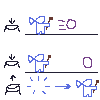
\includegraphics[scale=2.0]{img/cetro-esquema.png}
    \caption[Esquema de funcionamiento del cetro para el GDD]{Esquema de funcionamiento del cetro. Al pulsar el botón, aparece un marcador que va recorriendo cierta distancia. Mientras se mantenga pulsado, ese marcador permanecerá quieto aunque el jugador se mueva. Al soltarlo, el jugador aparece donde estaba el marcador.}
    \label{fig:cetro}
\end{figure}

\section{Estructura general del juego}

La estructura general del juego viene indicada en la Figura \ref{fig:structurediagram}. Esta va marcada por las mejoras a desbloquear, es decir, el orden en el que es necesario hacerlo.

\begin{figure}[h]
    \centering
    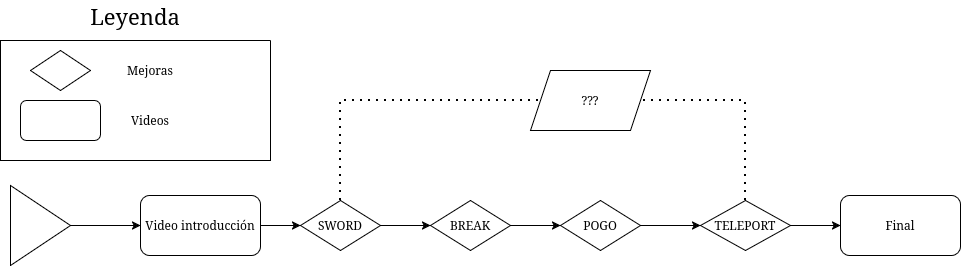
\includegraphics[scale=0.48]{img/game_structure.drawio.png}
    \caption[Estructura general del juego]{Estructura general del juego}
    \label{fig:structurediagram}
\end{figure}

\section{Características adicionales}

Aquí se enumeran a modo de cajón de sastre todas las características que no corresponden a la jugabilidad del proyecto:

\begin{itemize}
    \item El juego contará con una pantalla de título con opción a comenzar una nueva partida, cargar una anterior o salir. Se podrán tener hasta tres partidas guardadas en total.
    \item El jugador podrá pausar el juego en cualquier momento.
    \item Desde el menú de pausa se podrá regresar a la pantalla de título, abrir un menú de ajustes, o reanudar la partida.
    \item En el menú de ajustes se podrá ajustar el volumen de los distintos canales de audio (música y sonido), activar o desactivar la pantalla completa, y acceder a las opciones de accesibilidad.
    \item Durante el juego se podrá abrir el menú del mapa. Cuando esto se haga, el resto del juego estará pausado a efectos prácticos.
    \item El menú del mapa mostrará la ubicación actual del jugador, las salas exploradas y las salas de guardado visitadas aparecerán marcadas.
\end{itemize}

\section{Arte}

El juego emplea un estilo \textit{pixel art} de baja resolución. Por norma general, los personajes están encuadrados en una resolución de \textit{16x16 píxeles}. Se usarán colores planos vibrantes y llamativos sin abusar del contraste. Se usará iconografía sencilla y universal que prioriza la representación conceptual de un objeto que su calidad o técnica artística.

\subsection{Referencias visuales}


Se presentan ahora una serie de referencias visuales que ilustran el estilo general que busca tener el juego. Corresponden a las figuras \ref{fig:vvvvvv}, \ref{fig:fishivy}, \ref{fig:famulus} y \ref{fig:boborobo}.

\begin{figure}[h]
    \centering


    \begin{minipage}{0.45\textwidth}
        \centering
        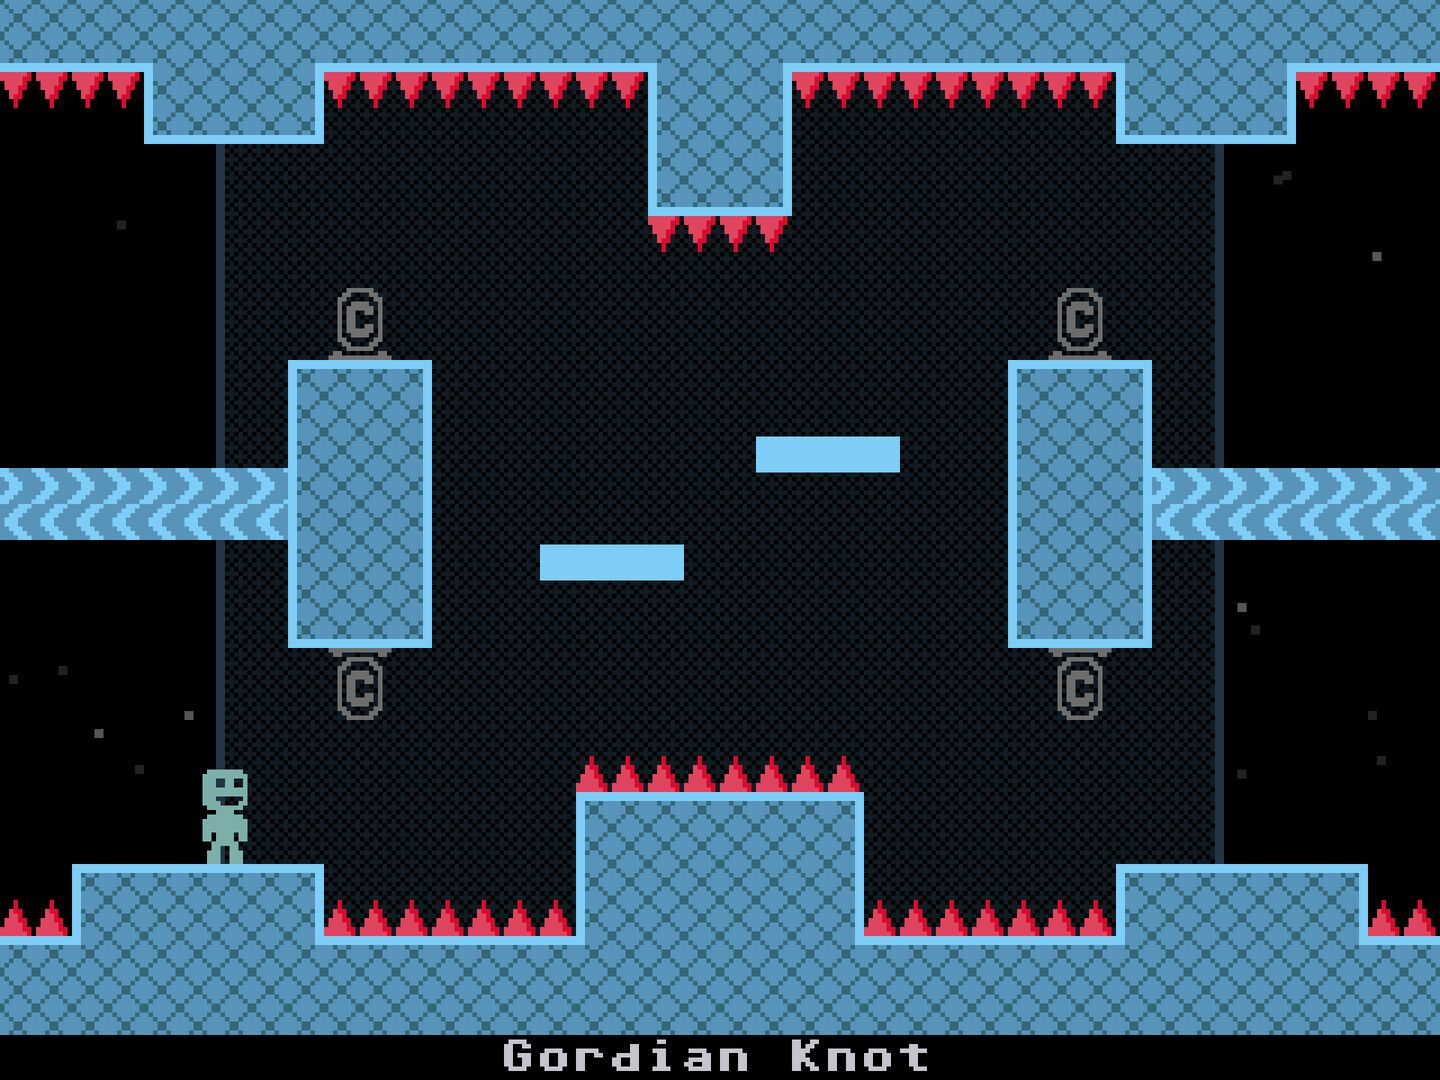
\includegraphics[width=\linewidth]{img/vvvvvv_1.jpg}
    \end{minipage}
    \hfill
    \begin{minipage}{0.45\textwidth}
        \centering
        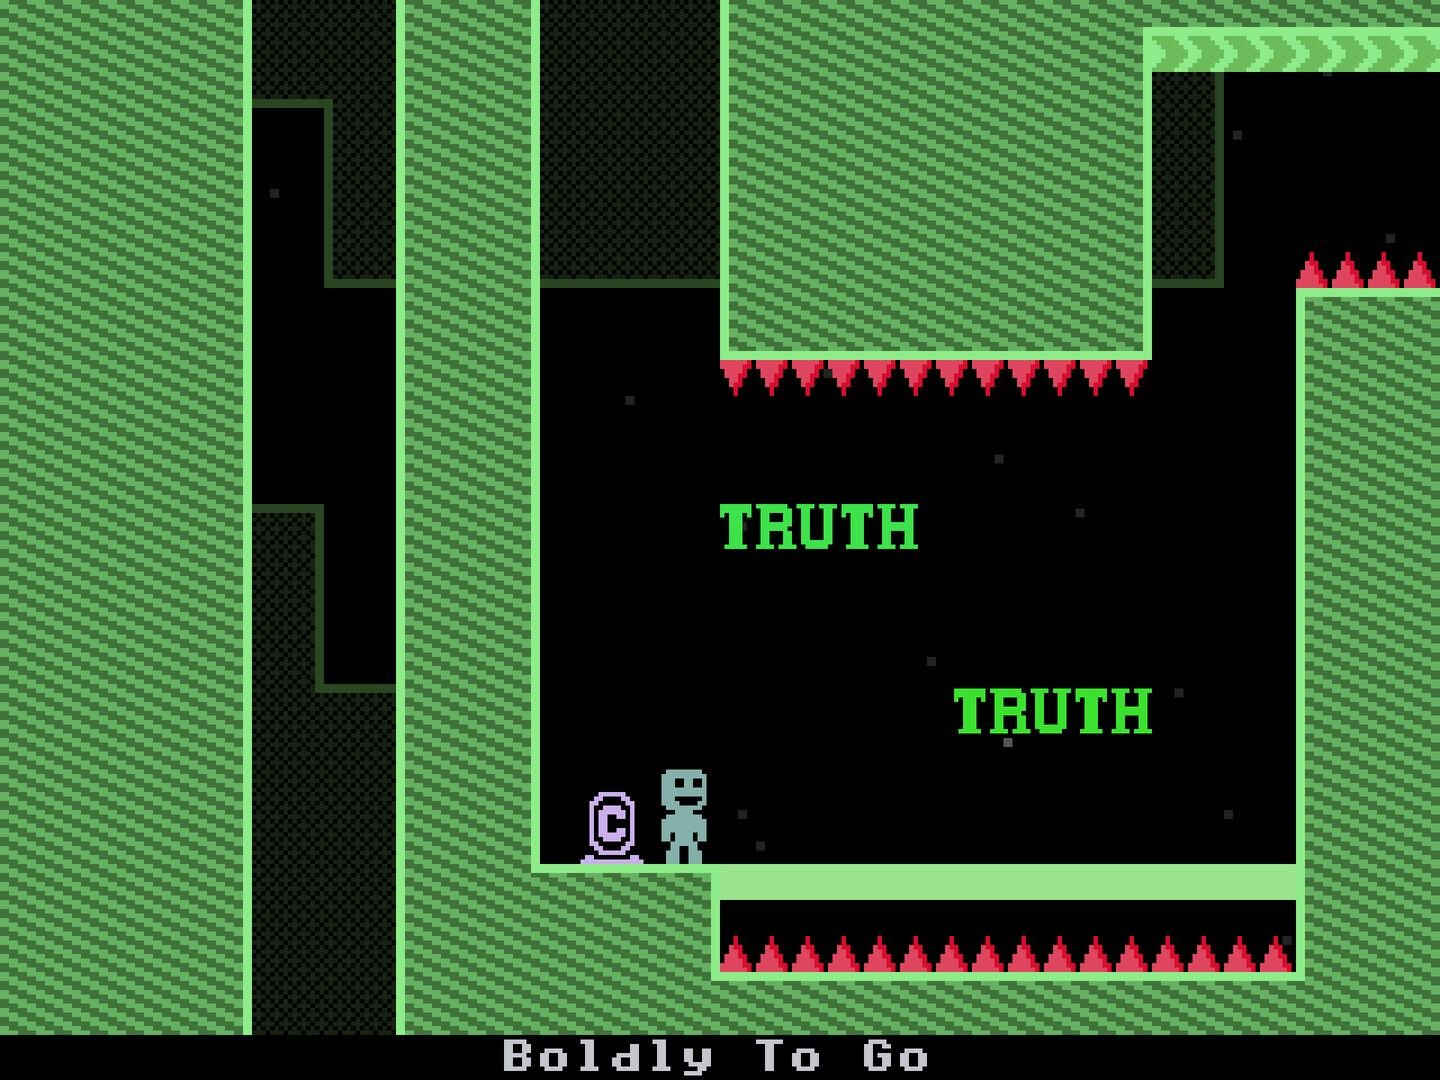
\includegraphics[width=\linewidth]{img/vvvvvv_2.jpg}
    \end{minipage}

    \vspace{0.4cm}

    \begin{minipage}{0.6\textwidth}
        \centering
        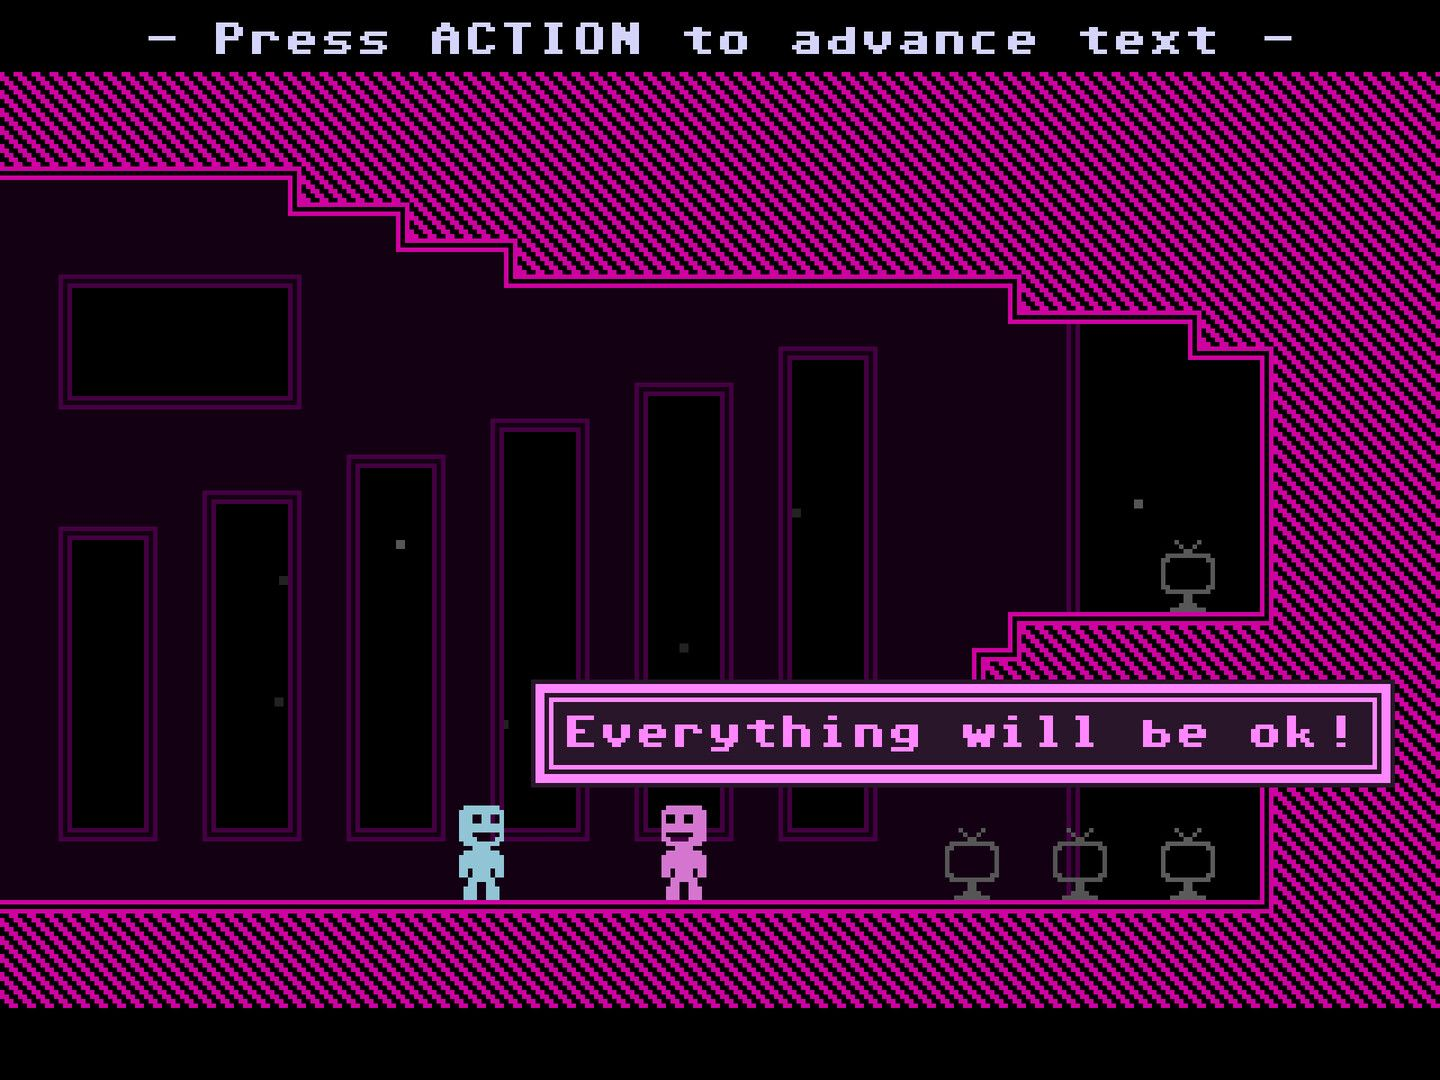
\includegraphics[width=\linewidth]{img/vvvvvv_3.jpg}
    \end{minipage}

    \caption[Referencia visual 1]{VVVVVV, Terry Cavanagh. Imágenes extraídas de \href{https://steamdeckhq.com/news/vvvvvv-2-4-brings-steam-deck-verified-badge/}{SteamDeckHQ}.}
    \label{fig:vvvvvv}
\end{figure}

\begin{figure}[h]
    \centering


    \begin{minipage}{0.45\textwidth}
        \centering
        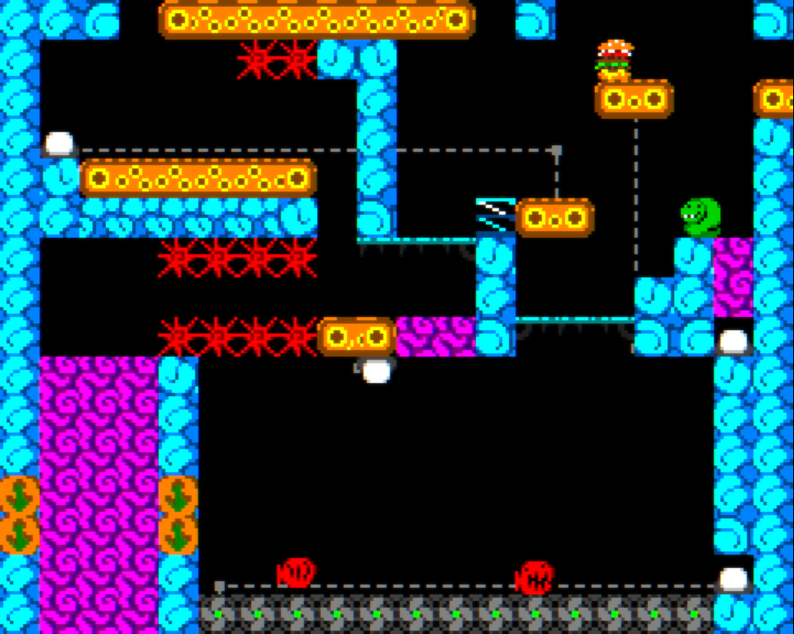
\includegraphics[width=\linewidth]{img/fish_1.png}
    \end{minipage}
    \hfill
    \begin{minipage}{0.45\textwidth}
        \centering
        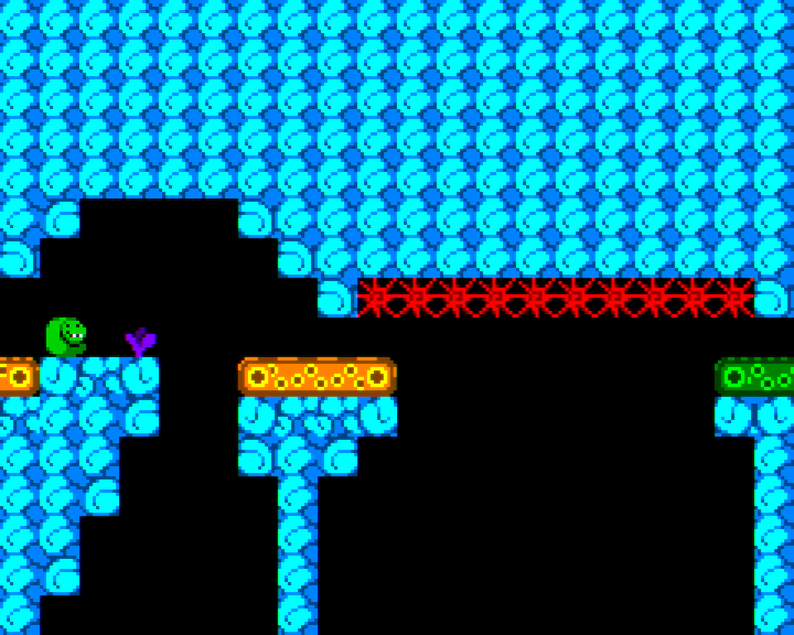
\includegraphics[width=\linewidth]{img/fish_2.png}
    \end{minipage}

    \vspace{0.4cm}

    \begin{minipage}{0.6\textwidth}
        \centering
        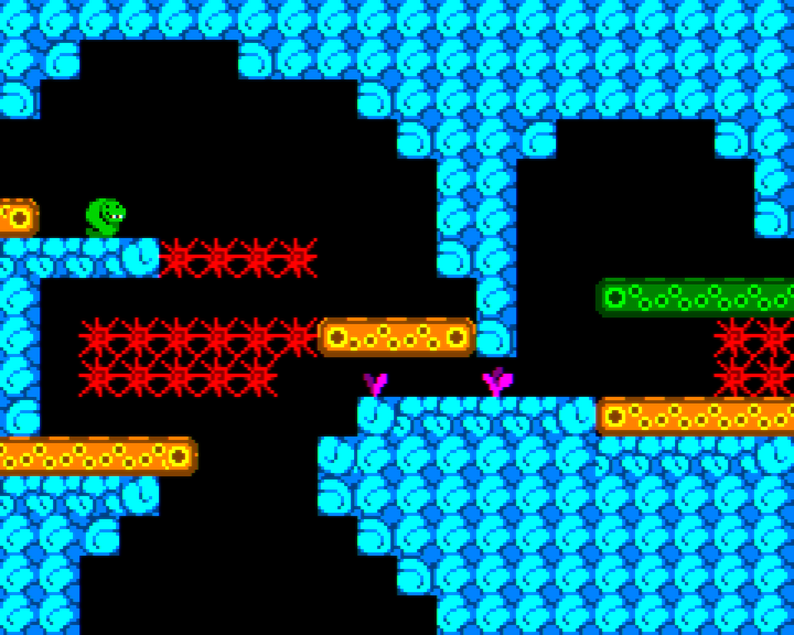
\includegraphics[width=\linewidth]{img/fish_3.png}
    \end{minipage}

    \caption[Referencia visual 2]{\textit{The Astonishing Adventures Of Finspector Eelliott Fishbone: Eel Detective Part 6: TRAPPED On Planet Big Burger!}, ivisly. Imágenes extraídas de \href{https://ivysly.itch.io/finspector-eelliott-fishbone-eel-detective-part-6-trapped-on-planet-big-burger}{Itch.io}.}
    \label{fig:fishivy}
\end{figure}

\begin{figure}[h]
    \centering


    \begin{minipage}{0.45\textwidth}
        \centering
        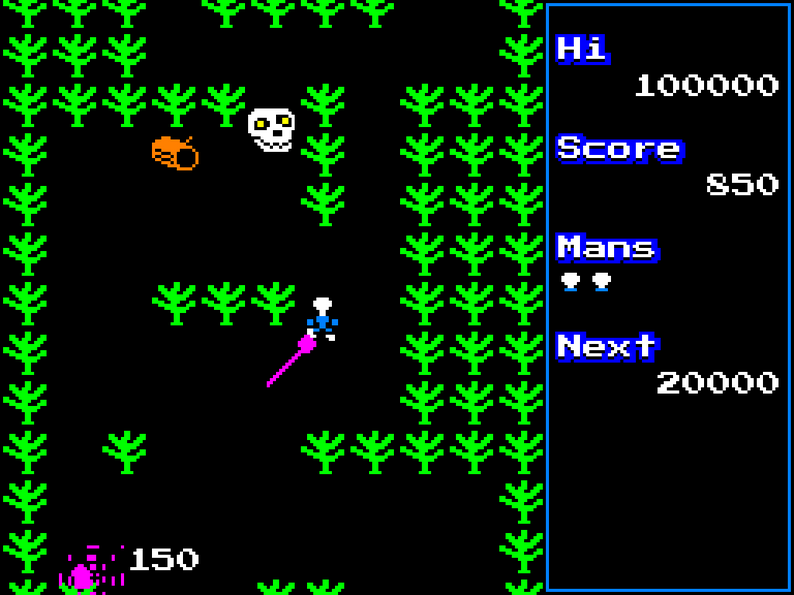
\includegraphics[width=\linewidth]{img/famulus_1.png}
    \end{minipage}
    \hfill
    \begin{minipage}{0.45\textwidth}
        \centering
        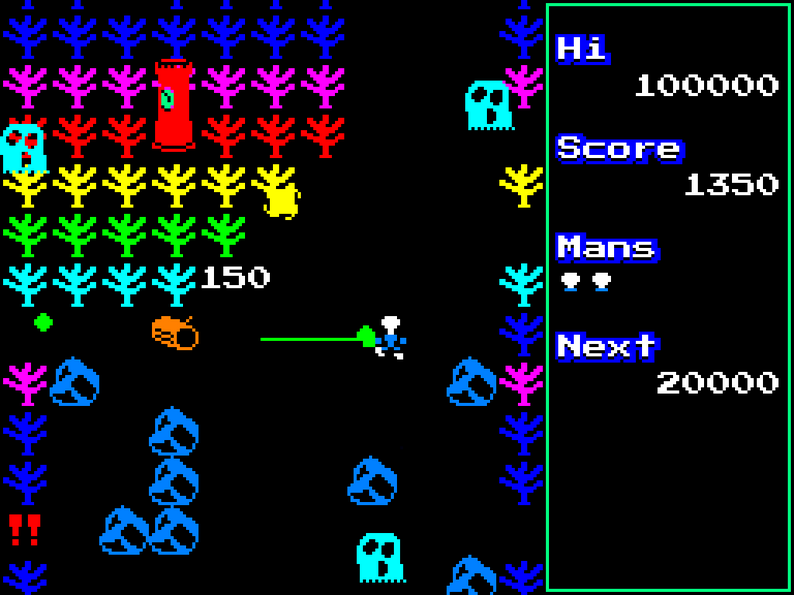
\includegraphics[width=\linewidth]{img/famulus_2.png}
    \end{minipage}

    \vspace{0.4cm}

    \begin{minipage}{0.6\textwidth}
        \centering
        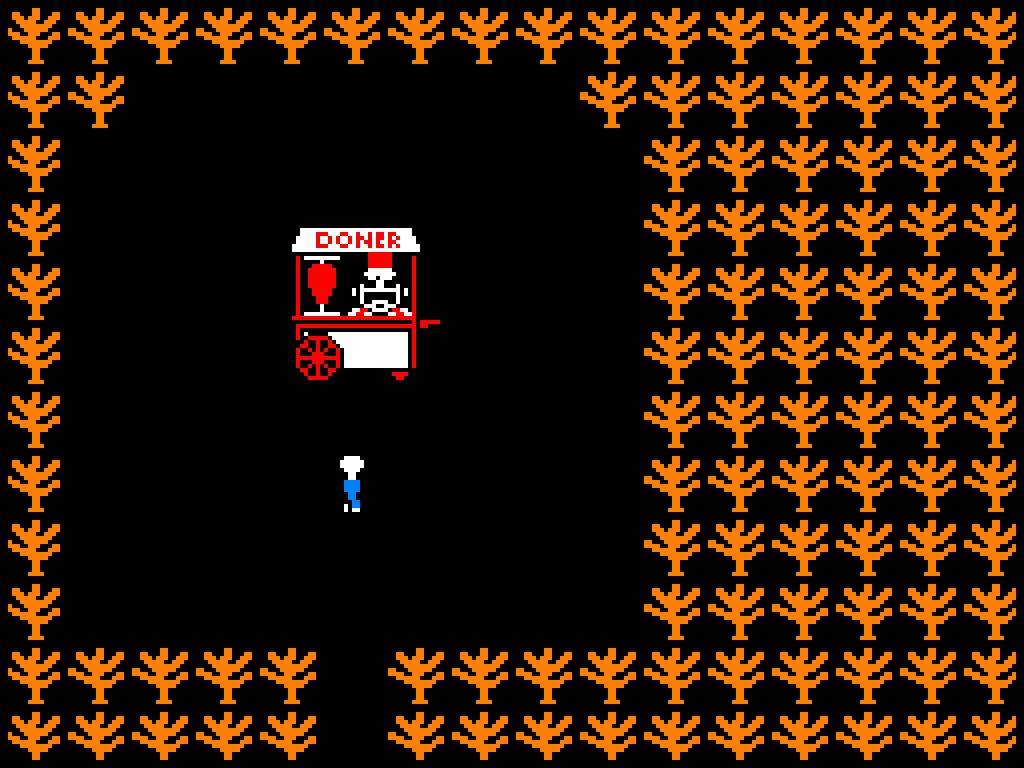
\includegraphics[width=\linewidth]{img/famulus_3.png}
    \end{minipage}

    \caption[Referencia visual 3]{\textit{Famulus}, ivisly. Imágenes extraídas de \href{https://ivysly.itch.io/famulus}{Itch.io}.}
    \label{fig:famulus}
\end{figure}

\begin{figure}[h]
    \centering


    \begin{minipage}{0.45\textwidth}
        \centering
        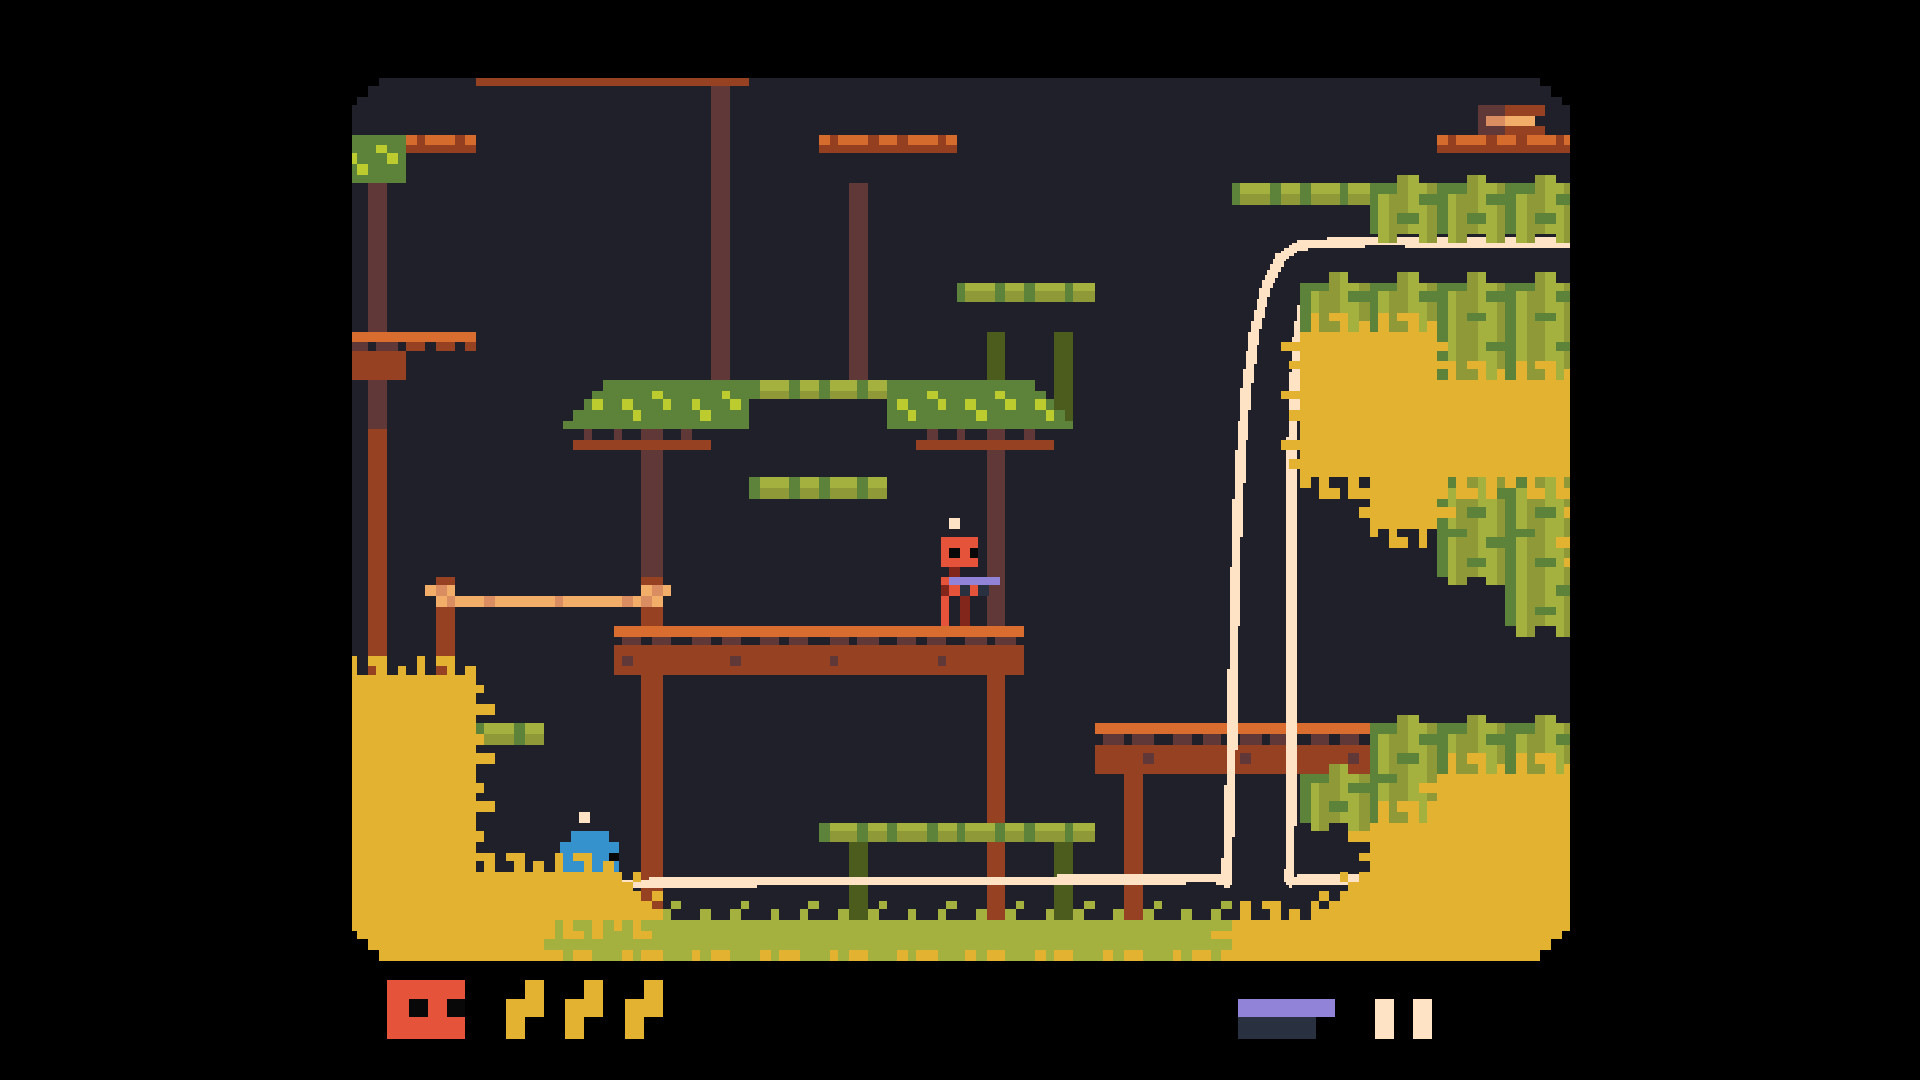
\includegraphics[width=\linewidth]{img/bobo_robo_1.jpg}
    \end{minipage}
    \hfill
    \begin{minipage}{0.45\textwidth}
        \centering
        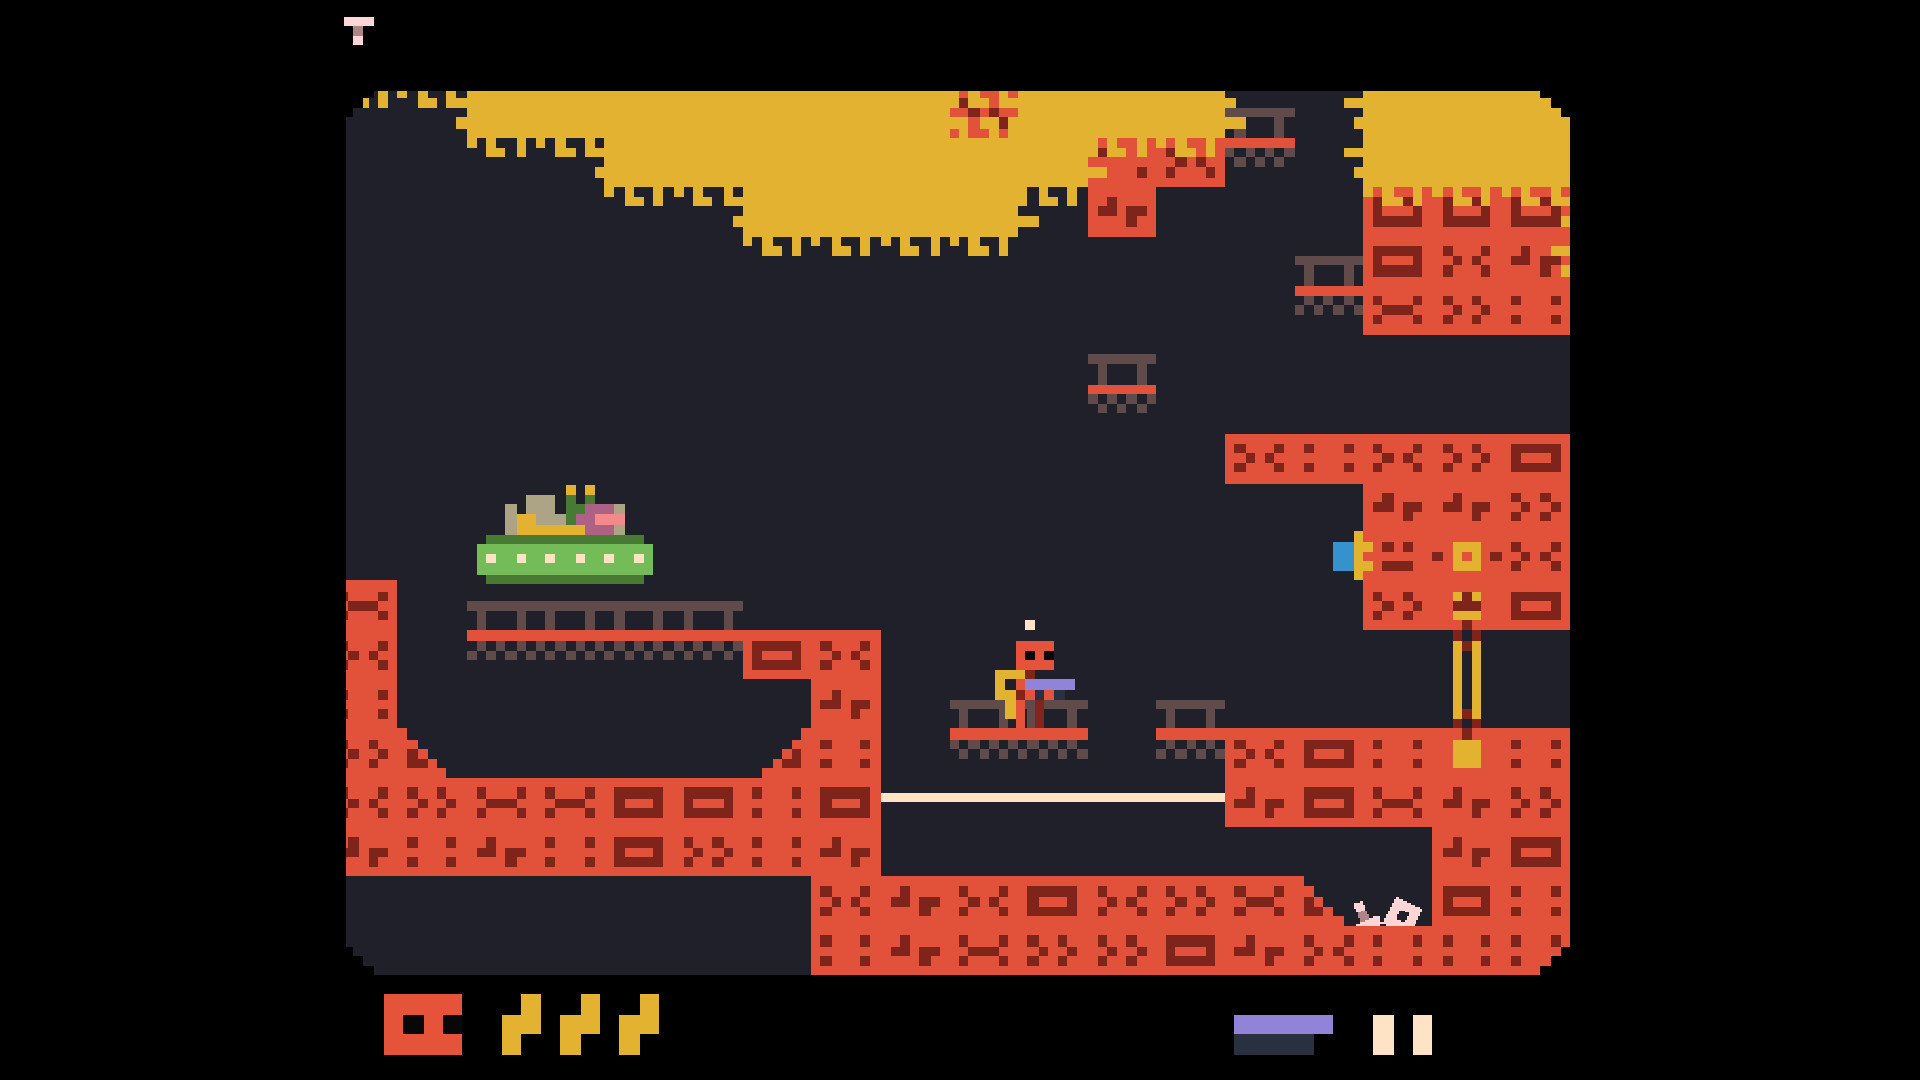
\includegraphics[width=\linewidth]{img/bobo_robo_2.jpg}
    \end{minipage}

    \vspace{0.4cm}

    \begin{minipage}{0.6\textwidth}
        \centering
        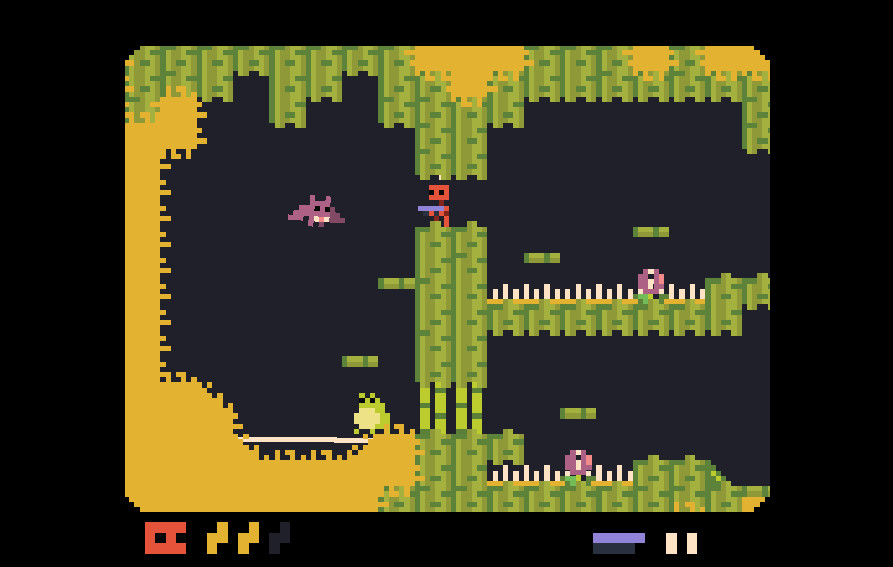
\includegraphics[width=\linewidth]{img/bobo_robo_3.jpg}
    \end{minipage}

    \caption[Referencia visual 4]{\textit{bobo robot}, Sokpop. Imágenes extraídas de \href{https://store.steampowered.com/app/1211540/bobo_robot/}{Steam}.}
    \label{fig:boborobo}
\end{figure}

\subsection{Arte conceptual}

El arte conceptual realizado durante la preproducción se puede observar en las figuras \ref{fig:boceto-pez}, \ref{fig:boceto-animacion-pez}, \ref{fig:boceto-personajes} y \ref{fig:boceto-level}.

\begin{figure}[h]
    \centering
    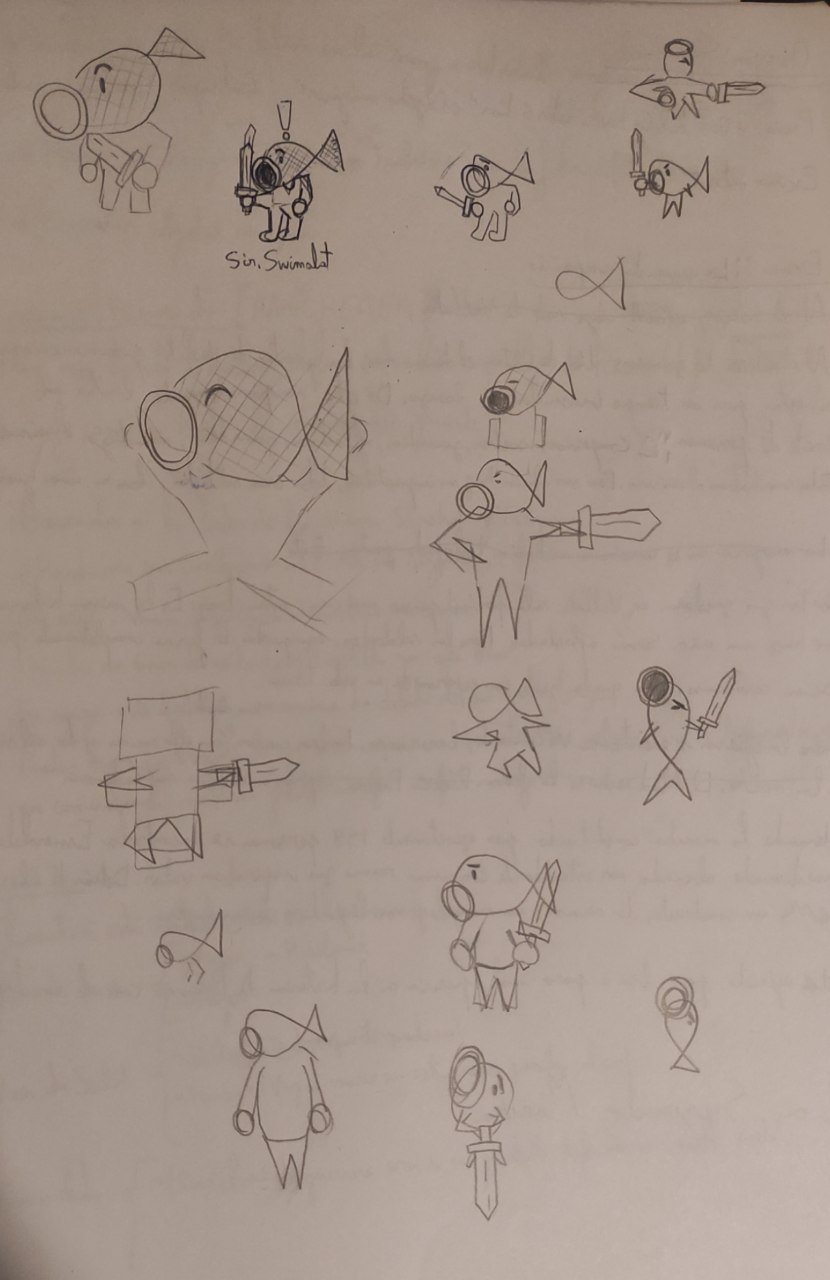
\includegraphics[scale=0.25]{img/boceto.jpg}
    \caption[Bocetos conceptuales a papel realizados en preproducción]{Bocetos conceptuales a papel realizados en preproducción}
    \label{fig:boceto-pez}
\end{figure}

\begin{figure}[h]
    \centering
    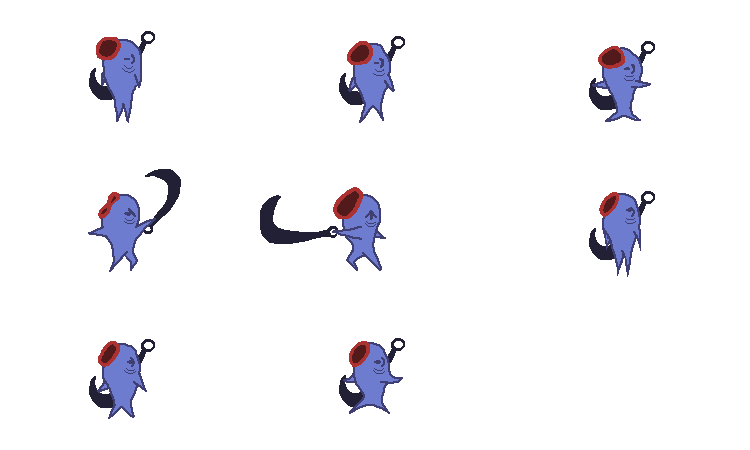
\includegraphics[scale=0.5]{img/mockup-animation.png}
    \caption[Boceto conceptual animado de personaje principal]{Boceto conceptual animado de personaje principal con acciones básicas como correr, saltar y atacar.}
    \label{fig:boceto-animacion-pez}
\end{figure}

\begin{figure}[h]
    \centering
    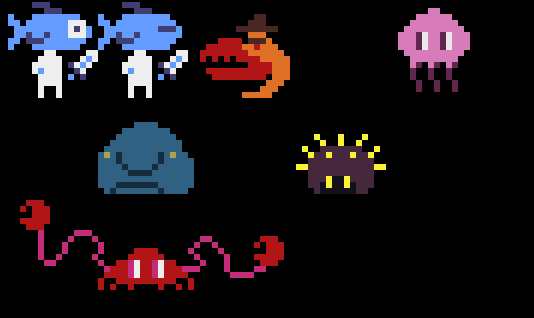
\includegraphics[scale=0.5]{img/mockup-characters.png}
    \caption[Bocetos conceptuales de personaje jugador y enemigos en baja resolución]{Bocetos conceptuales de personaje jugador y enemigos en baja resolución}
    \label{fig:boceto-personajes}
\end{figure}

\begin{figure}[h]
    \centering
    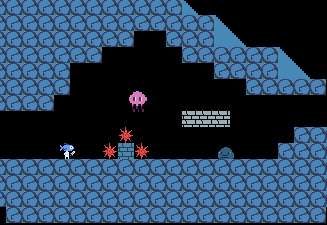
\includegraphics[scale=0.7]{img/screen-mockup.png}
    \caption[Bocetos conceptuales de simulación de nivel]{Bocetos conceptual de simulación de nivel}
    \label{fig:boceto-level}
\end{figure}

